%!TEX root = ../../../main.tex

\section{Introduction}

\begin{frame}{What does ``Model-Checking'' mean?}
\only<1> {
  \centerline{
\includegraphics[width=.8\textwidth]{content/chapter_model_checking/model_checking/images/models}}
}

\only<2> {
  \centerline{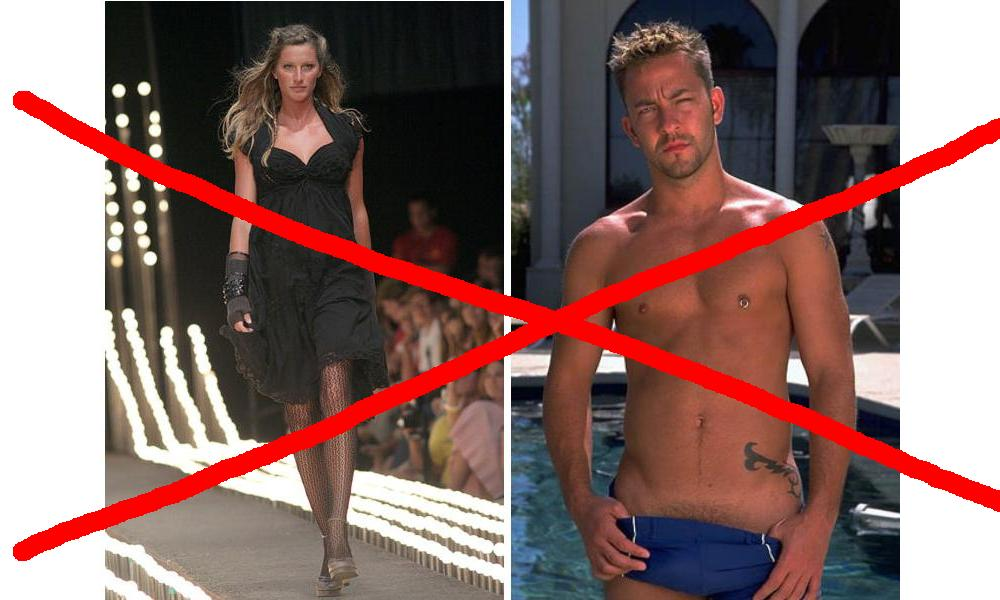
\includegraphics[width=\textwidth]{content/chapter_model_checking/model_checking/images/models1}}
}

\only<3-> {
  \begin{itemize}
    \item \hl{A technical term from logic}
    \item Temporal logic: extension of predicate logic
    \item In german: ``Modellpr"ufung'' (rarely used)
  \end{itemize}
}
\end{frame}

% ----------------------------------------------------------------------

\begin{frame}{Propositional logic (Syntax)}
Formulae of propositional logic consist of \hl{atomic propositions}, e.g.
\bigskip
\begin{itemize}
  \itemsep1em
  \item[] $\mathbf{A}$ \quad $\widehat=$ \quad ``Anna is an architect''
  \item[] $\mathbf{B}$ \quad $\widehat=$ \quad ``Bruno is a bear''
\end{itemize}
\bigskip
and \hl{connectives}, e.g.\ $\land$ (``and''),
    $\lor$ (``or''), $\neg$ (``not''),
    $\to$ (``implies'').
\end{frame}

% ----------------------------------------------------------------------

\begin{frame}{Semantics of propositional logic}

A \hl{valuation} $\mathcal{B}$ is a function assigning 
a \hl{truth value} (\hl{1} or \hl{0}) to each atomic proposition.

\bigskip
The \hl{semantics} of a formula (defined inductively) is the set of valuations
making the formula ``true'' and denoted $\sema{F}$.

\begin{itemize}
  \item[] if \m{F=A} then \m{\sema{F}=\{\,\mathcal{B}\mid\mathcal{B}(A)=1\,\}};
  \item[] if \m{F=F_1 \land F_2} then \m{\sema{F}=\sema{F_1}\cap\sema{F_2}}; \ldots
\end{itemize}

\bigskip
Other notations: $\mathcal{B}\models F$ iff $\mathcal{B}\in\sema{F}$.\\
We say: ``\m{\mathcal{B}} fulfils \m{F}'' or ``\m{\mathcal{B}} is a model of \m{F}''.
\end{frame}

% ----------------------------------------------------------------------

\begin{frame}{The model-checking problem in propositional logic}
\hl{Problem:} Given a valuation \m{\mathcal{B}}
   and a formula \m{F} of propositional logic;

\begin{center}
check whether \m{\mathcal{B}} is a model of \m{F}.
\end{center}   


\hl{Solution}:
\begin{quote}
Replace the atomic propositions by their truth values in \m{\mathcal{B}},
then use a truth table to evaluate to \m{1} or \m{0}.
\end{quote}

\bigskip
\hl{Examples:} 
\begin{itemize}
  \item Let \m{\mathcal{B}_1(A)=1} and \m{\mathcal{B}_1(B)=0}.
  Then \m{\mathcal{B}_1\not\models A\land B} and \m{\mathcal{B}_1\models\neg B}

  \item Let \m{\mathcal{B}_2(A)=1} and \m{\mathcal{B}_2(B)=1}. 
  Then \m{\mathcal{B}_2\models A\land B} and \m{\mathcal{B}_2\not\models\neg B}.
\end{itemize}

\end{frame}

% ----------------------------------------------------------------------

\begin{frame}{Temporal logic}

Takes into account that truth values of atomic proposition may
change with time (the ``world'' transforms).

\bigskip
Example: Truth values of \m{A} in the course of Anna's life:

\begin{center}
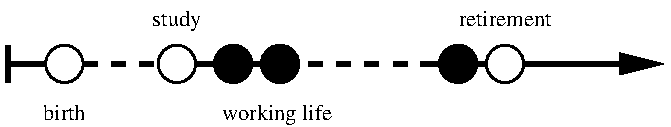
\includegraphics[width=\textwidth]{content/chapter_model_checking/model_checking/images/anna}
\end{center}

Possible statements:
\begin{itemize}
\item Anna will \hl{eventually} be an architect (at some point in the future).
\item Anna is an architect \hl{until} she retires.
\end{itemize}
$\Longrightarrow$ Extension of propositional logic with
    temporal connectives (eventually, until)
\end{frame}

% ----------------------------------------------------------------------

\begin{frame}{Preview}
\hl{Linear-time temporal logics} (example: LTL)
\begin{itemize}
\item formulae with temporal operators
\item evaluated w.r.t.\ (infinite) sequences of valuations
\item Model-checking problem for LTL: Given an LTL formula and a
   sequence of valuations, check whether the sequence is a model
   of the formula.
\end{itemize}

\bigskip
\hl{Computation-tree logic} (CTL, CTL${}^*$)
\begin{itemize}
\item Considers (infinite) \emph{trees} of valuations.
\item Interpretation: non-determinism; multiple possible developments.
\end{itemize}

\end{frame}

% ----------------------------------------------------------------------

\begin{frame}{Connection with program verification}

\hl{State space} of a program:
\begin{itemize}
\item value of program counter
\item contents of variables
\item contents of stack, heap, \ldots
\end{itemize}

\bigskip
Possible atomic propositions:
\begin{itemize}
\item ``Variable $x$ has a positive value.''
\item ``The program counter is at label~$\ell$.''
\end{itemize}

\bigskip
Given a set of atomic propositions, each program state gives rise to a valuation!

\end{frame}

% ---------------------------------------------------------------------- 

\begin{frame}{Programs and temporal logics}

\hl{Linear-time temporal logic}:
\begin{itemize}
\item Each program execution yields a \hl{sequence} of valuations.
\item Interpretation of the program: the set of possible sequences
\item Question of interest: Do all sequences satisfy a given LTL formula?
\end{itemize}

\bigskip
\hl{Computation-tree logic}:
\begin{itemize}
\item The program may branch at certain points, its possible executions
   yield a \hl{tree} of valuations.
\item Interpretation of the program: tree with the (valuation of the)
   initial state as its root
\item Question of interest: Does this tree satisfy a given CTL formula?
\end{itemize}

\bigskip
Thus:
\begin{center}
\hl{verification problem} \ \ $\widehat=$ \ \ \hl{model-checking problem}
\end{center}

\end{frame}


% ----------------------------------------------------------------------

\begin{frame}{Model checking}

Apart from its definition in terms of logic, the term \hl{model checking} is generally understood to mean methods that
\begin{itemize}
\item \hl{verify} whether a given system satisfies a given specification;
\item work \hl{automatically};
\item either prove \hl{correctness} of the system w.r.t.\ to the specification;
\item or exhibit a \hl{counterexample}, i.e.\ an execution violating the
   specification (at least in the linear-time framework).
\end{itemize}

\end{frame}

% ----------------------------------------------------------------------

\begin{frame}{Pros and cons of model checking}

\hl{Advantages:}
\begin{itemize}
\item works automatically(!)
\item suitable for reactive, concurrent, distributed systems
\item can check temporal-logic properties, not just reachability
\end{itemize}

\bigskip
\hl{Disadvantages:}
\begin{itemize}
  \item programs are Turing powerful $\rightarrow$ \hl{undecidability}
    Solution: consider decidable sub-classes
  
  \item state space is huge $\rightarrow$ \hl{computationally expensive}
    Solution: efficient data structures and algorithms
\end{itemize}
\end{frame}

% ----------------------------------------------------------------------

\begin{frame}{Problems with model checking}

  \begin{itemize}
    \item For the aforementioned problems we cannot hope to verify arbitrary
   properties of arbitrary programs!

    \item Possibly we must consider a simplified mathematical model of the system
   of interest that ignores its ``unimportant'' aspects.

    \item Construction of such models and the specification as well as the actual
   verification require \hl{effort} and (possibly high) \hl{cost}.

    \item $\Rightarrow$ useful in early design phases

    \item $\Rightarrow$ economic gain for critical systems where failure is
   costly (CPUs, communication protocols, aircraft, \ldots)
  \end{itemize}
\end{frame}


